% LaTeX Written Report for Evolutionary Robotics Final Project
\documentclass[12pt]{article}
\usepackage[left=1in, right=1in, top=0.75in, bottom=0.75in]{geometry}
\usepackage{setspace}
\usepackage{graphicx}
\usepackage{booktabs}
\usepackage{hyperref}
\usepackage{amsmath}
\usepackage{caption}
\usepackage{float}
\usepackage{subcaption}
\usepackage{titlesec}
\usepackage{titling}

% Title formatting
\pretitle{\begin{center}\Large\bfseries}
\posttitle{\\[0.5em]}
\preauthor{\large\begin{tabular}{c}}
\postauthor{\end{tabular}\end{center}}
\predate{\begin{center}\large}
\postdate{\end{center}}

\doublespacing
\begin{document}

% Custom title page
\begin{titlepage}
  \centering
  {\huge\bfseries Strength in Numbers: A/B Testing of Swarm Fitness Evaluation\par}
  \vspace{1.5cm}
  {\Large Aaron Perkel\par}
  {\emph{Evolutionary Robotics Final Project}\par}
  \vfill
  {\large May 5, 2025\par}
\end{titlepage}

% Table of Contents
\tableofcontents
\clearpage

\section{Goals}
This project extends my four‐legged robot deliverables into a swarm context and investigates two fitness evaluation methods.  

\begin{itemize}
  \item \textbf{Deliverables recap}:  
    \begin{enumerate}
      \item Multi‐URDF output for swarm members (Milestone 1)  
      \item Swarm simulation with obstacles (Milestones 2 and 3)  
      \item A/B testing framework comparing max‐based vs avg‐based selection (Milestone 4)  
    \end{enumerate}
  \item \textbf{A vs B variants}:  
    \begin{itemize}
      \item \emph{A}: max(distance) across swarm drives selection.  
      \item \emph{B}: average(distance) across swarm drives selection.  
    \end{itemize}
  \item \textbf{Research question}: Under what conditions does selecting the best individual outperform using the swarm’s average distance?  
\end{itemize}
\newpage

\section{Implementation}
I built on the existing repo to enable swarm‐based evaluation and automate the A/B tests.  

\begin{itemize}
  \item \textbf{Body generation (solution.py)}: wrote out multiple \texttt{body\_*.urdf} files with per-robot position offsets.
  \item \textbf{Simulation harness (simulate.py \& robot.py)}: loaded all URDFs in \texttt{src/data/}, ran PyBullet steps, and collected each robot’s x-position each timestep.
  \item \textbf{Fitness writer (robot.Get\_Fitness)}: computed both max and average distances, wrote \texttt{fitness\_max<ID>.txt} and \texttt{fitness\_avg<ID>.txt}, then renamed the chosen metric based on the \texttt{FITNESS\_METHOD} environment variable.
  \item \textbf{Automation scripts}:
    \begin{itemize}
      \item \texttt{run\_ab.sh} to launch 50 replicates per method and gather \texttt{fitness\_ab\_test.csv}.
      \item \texttt{abtest.py} for statistical analysis (two-sample t-tests) and box-plot generation.
    \end{itemize}
\end{itemize}


% Force table and plots on same page
\section{Results}
I ran nine experimental configurations (Table~\ref{tab:ab_results}) and evaluated significance at $\alpha = 0.05$.  

\begin{table}[H]
  \centering
  \caption{Summary of A/B test results across experiments}
  \label{tab:ab_results}
  \begin{tabular}{@{}lcccccccc@{}}
    \toprule
    Exp & Obstacles? & Reps & Steps & Pop & Swarm & Max mean & Avg mean & p-value \\
    \midrule
    a & Yes & 50 & 2500 & 2 & 2 & 1.269 & 0.495 & 0.0130 \\
    b & Yes & 50 & 5000 & 4 & 2 & 1.549 & 0.940 & 0.1975 \\
    c & Yes & 50 & 1000 & 2 & 2 & 0.942 & 0.593 & 0.0377 \\
    d & No  & 50 & 2500 & 5 & 5 & 0.802 & 0.174 & 0.0343 \\
    e & No  & 50 & 1000 & 2 & 2 & 0.225 & -0.036 & 0.1929 \\
    f & Yes & 25 & 1000 & 2 & 1 & -0.096 & 0.399 & 0.0512 \\
    g & Yes & 50 & 2000 & 3 & 3 & 1.158 & 0.243 & 0.0009 \\
    h & No  & 50 & 2000 & 2 & 3 & 0.748 & 0.269 & 0.1220 \\
    i & Yes & 50 & 3000 & 4 & 4 & 0.908 & 0.532 & 0.1760 \\
    \bottomrule
  \end{tabular}
\end{table}

\begin{figure}[H]
  \centering
  \begin{subfigure}[t]{0.45\textwidth}
    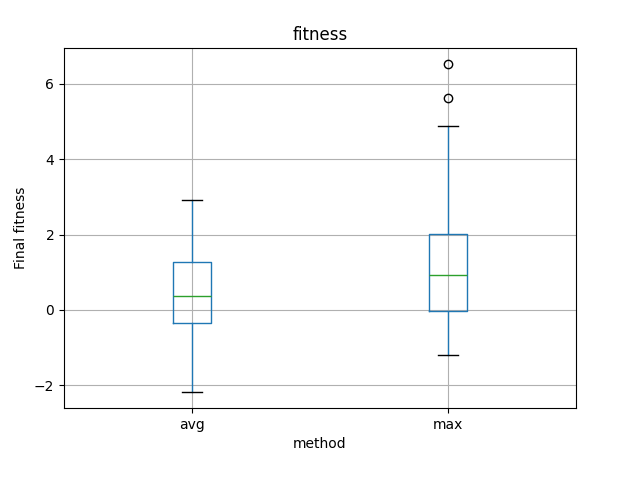
\includegraphics[width=\textwidth]{img/fig_a_boxplot.png}
    \caption{Experiment a}
  \end{subfigure}
  \begin{subfigure}[t]{0.45\textwidth}
    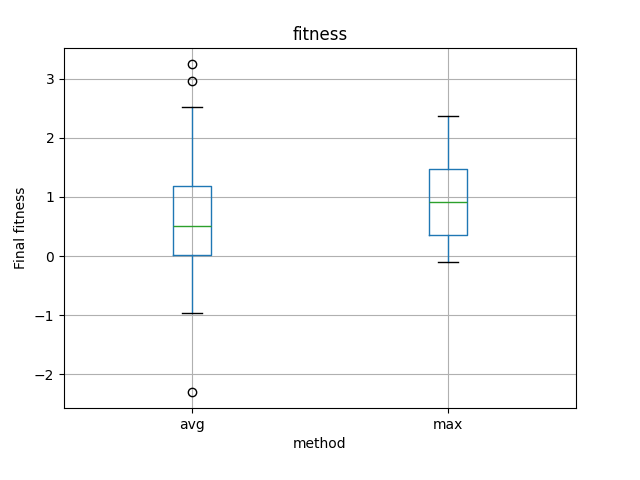
\includegraphics[width=\textwidth]{img/fig_c_boxplot.png}
    \caption{Experiment c}
  \end{subfigure}\\[0.5em]
  \begin{subfigure}[t]{0.45\textwidth}
    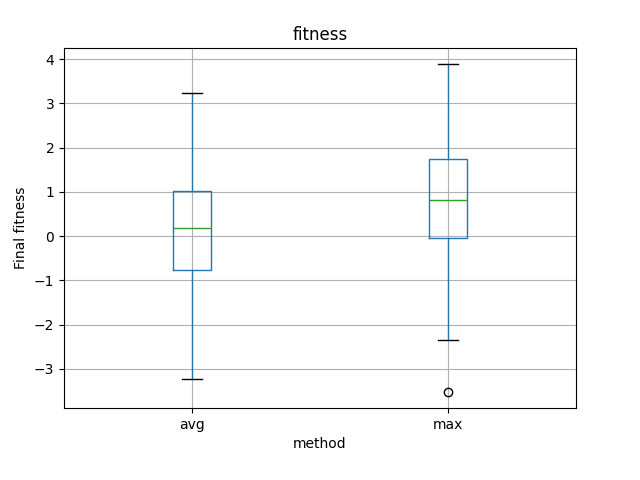
\includegraphics[width=\textwidth]{img/fig_d_boxplot.png}
    \caption{Experiment d}
  \end{subfigure}
  \begin{subfigure}[t]{0.45\textwidth}
    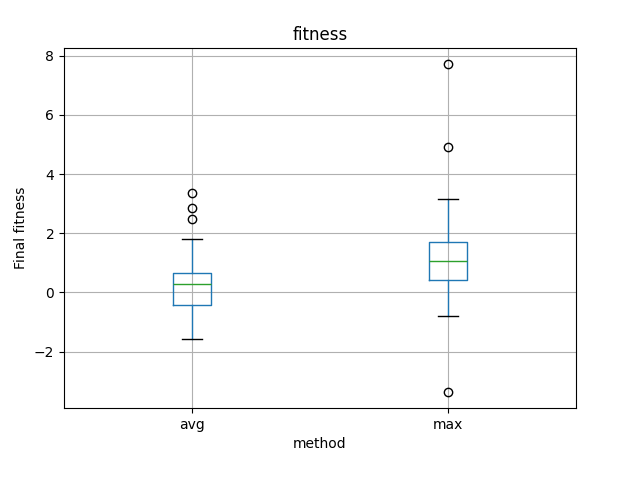
\includegraphics[width=\textwidth]{img/fig_g_boxplot.png}
    \caption{Experiment g}
  \end{subfigure}
  \caption{Key experiments where max-based selection was significant (a, c, d, g).}
  \label{fig:grid_boxplots}
\end{figure}

\section{Discussion \& Future Work}
\textbf{Ease and difficulty:} Adapting the fitness writer and automation scripts was straightforward; handling asynchronous simulation outputs and cleanup required careful file‐watching logic.  

\textbf{Patterns and Conclusions:}
\begin{enumerate}
  \item Obstacles + moderate size → “max” wins decisively (a, c, g).
  \item No obstacles → “max” rarely helps (d marginally; e, h non-significant).
  \item High budgets (lots of steps or generations) or large swarms/populations → the advantage of rewarding only the best performer fades (b, i).
  \item Single-robot “swarms” collapse to no difference (f).
\end{enumerate}

\textbf{Future directions:}
\begin{itemize}
  \item Introduce dynamic obstacles, varied terrain, or moving hazards to stress‐test swarm coordination.  
  \item Enhance Pyrosim with built‐in swarm primitives.
  \item Scale to larger swarm sizes.  
\end{itemize}

\end{document}